\chapter{数据采集方案与被试人口信息学特征统计}
\section{引言}
数据是一切分析的基础与前提,如何获取有效可靠的数据源是本研究亟需解决的问题。由于目前暂无公开可用的PE生理信号数据库,本研究最终选择自主设计采集实验以获取所需数据。
本章首先阐述了本研究的临床数据采集方案,对实验过程中涉及的被试人员筛选标准、生理数据采集规范及数据导出流程等问题进行了介绍。此外,本章也完成了被试人员的脉搏波外的人口信息学特征数据进行了基本的相关性分析工作。
\section{数据采集方案设计}
为获取足量脉搏波数据,本研究于2017年6月至2019年4月期间于浙江大学附属妇产科医院进行了数据采集实验。其中,患有PE的孕妇的PPG数据做为此次实验的实验组,而正常妊娠孕妇的PPG数据则做为对照组。
数据采集实验经过浙江大学附属妇产科医院医学伦理委员会的审查并被批准进行(审查编号:20140047)。所有参与实验的孕妇均在知晓本研究目的及具体实验流程的情况下同意参与其中。
需特别引起注意的是,所有实验组孕妇均已确诊PE,出现不同程度的血压升高在内的临床症状。因此,\textbf{实验组所有患有PE的孕妇均已接受过药物治疗在内的临床干预以减轻其症状}。
\subsection{实验设备}
本研究对脉搏波数据采集仪器的专业性、可靠性都有较高要求。在考察实验场地(浙江大学附属妇产科医院麻醉科室)的诸多临床在用设备后,最后选取了美国GE公司生产的GE Healthcare CARESCAPE B650 麻醉监护仪进行数据采集。
B650监护仪可对包括12导联心电、脑电、心输出量、血氧饱和度、血压、呼出气体中$CO_{2}$与$O_{2}$成份及熵指数等专业参数进行监测,如\autoref{fig:monitor}所示。此外,B650监护仪还提供了基于血氧的表征动脉血压变化的
收缩压变化参数(Systolic pressure variation,SPV)和脉压变化参数(pulse pressure variation,PPV)\cite{GE2021,Michard1999}。
\begin{figure}[htbp]
      \centering
      \subfigure[B650监护仪及其配件]{
      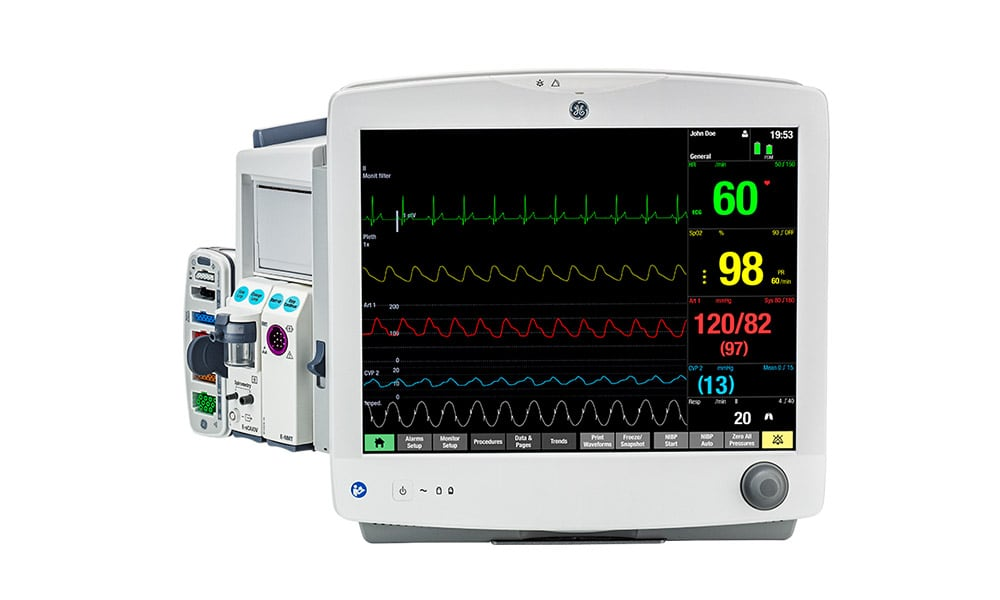
\includegraphics[width=7cm]{data_plan/monitor1}
      }
      \quad
      \subfigure[B650监护界面]{
      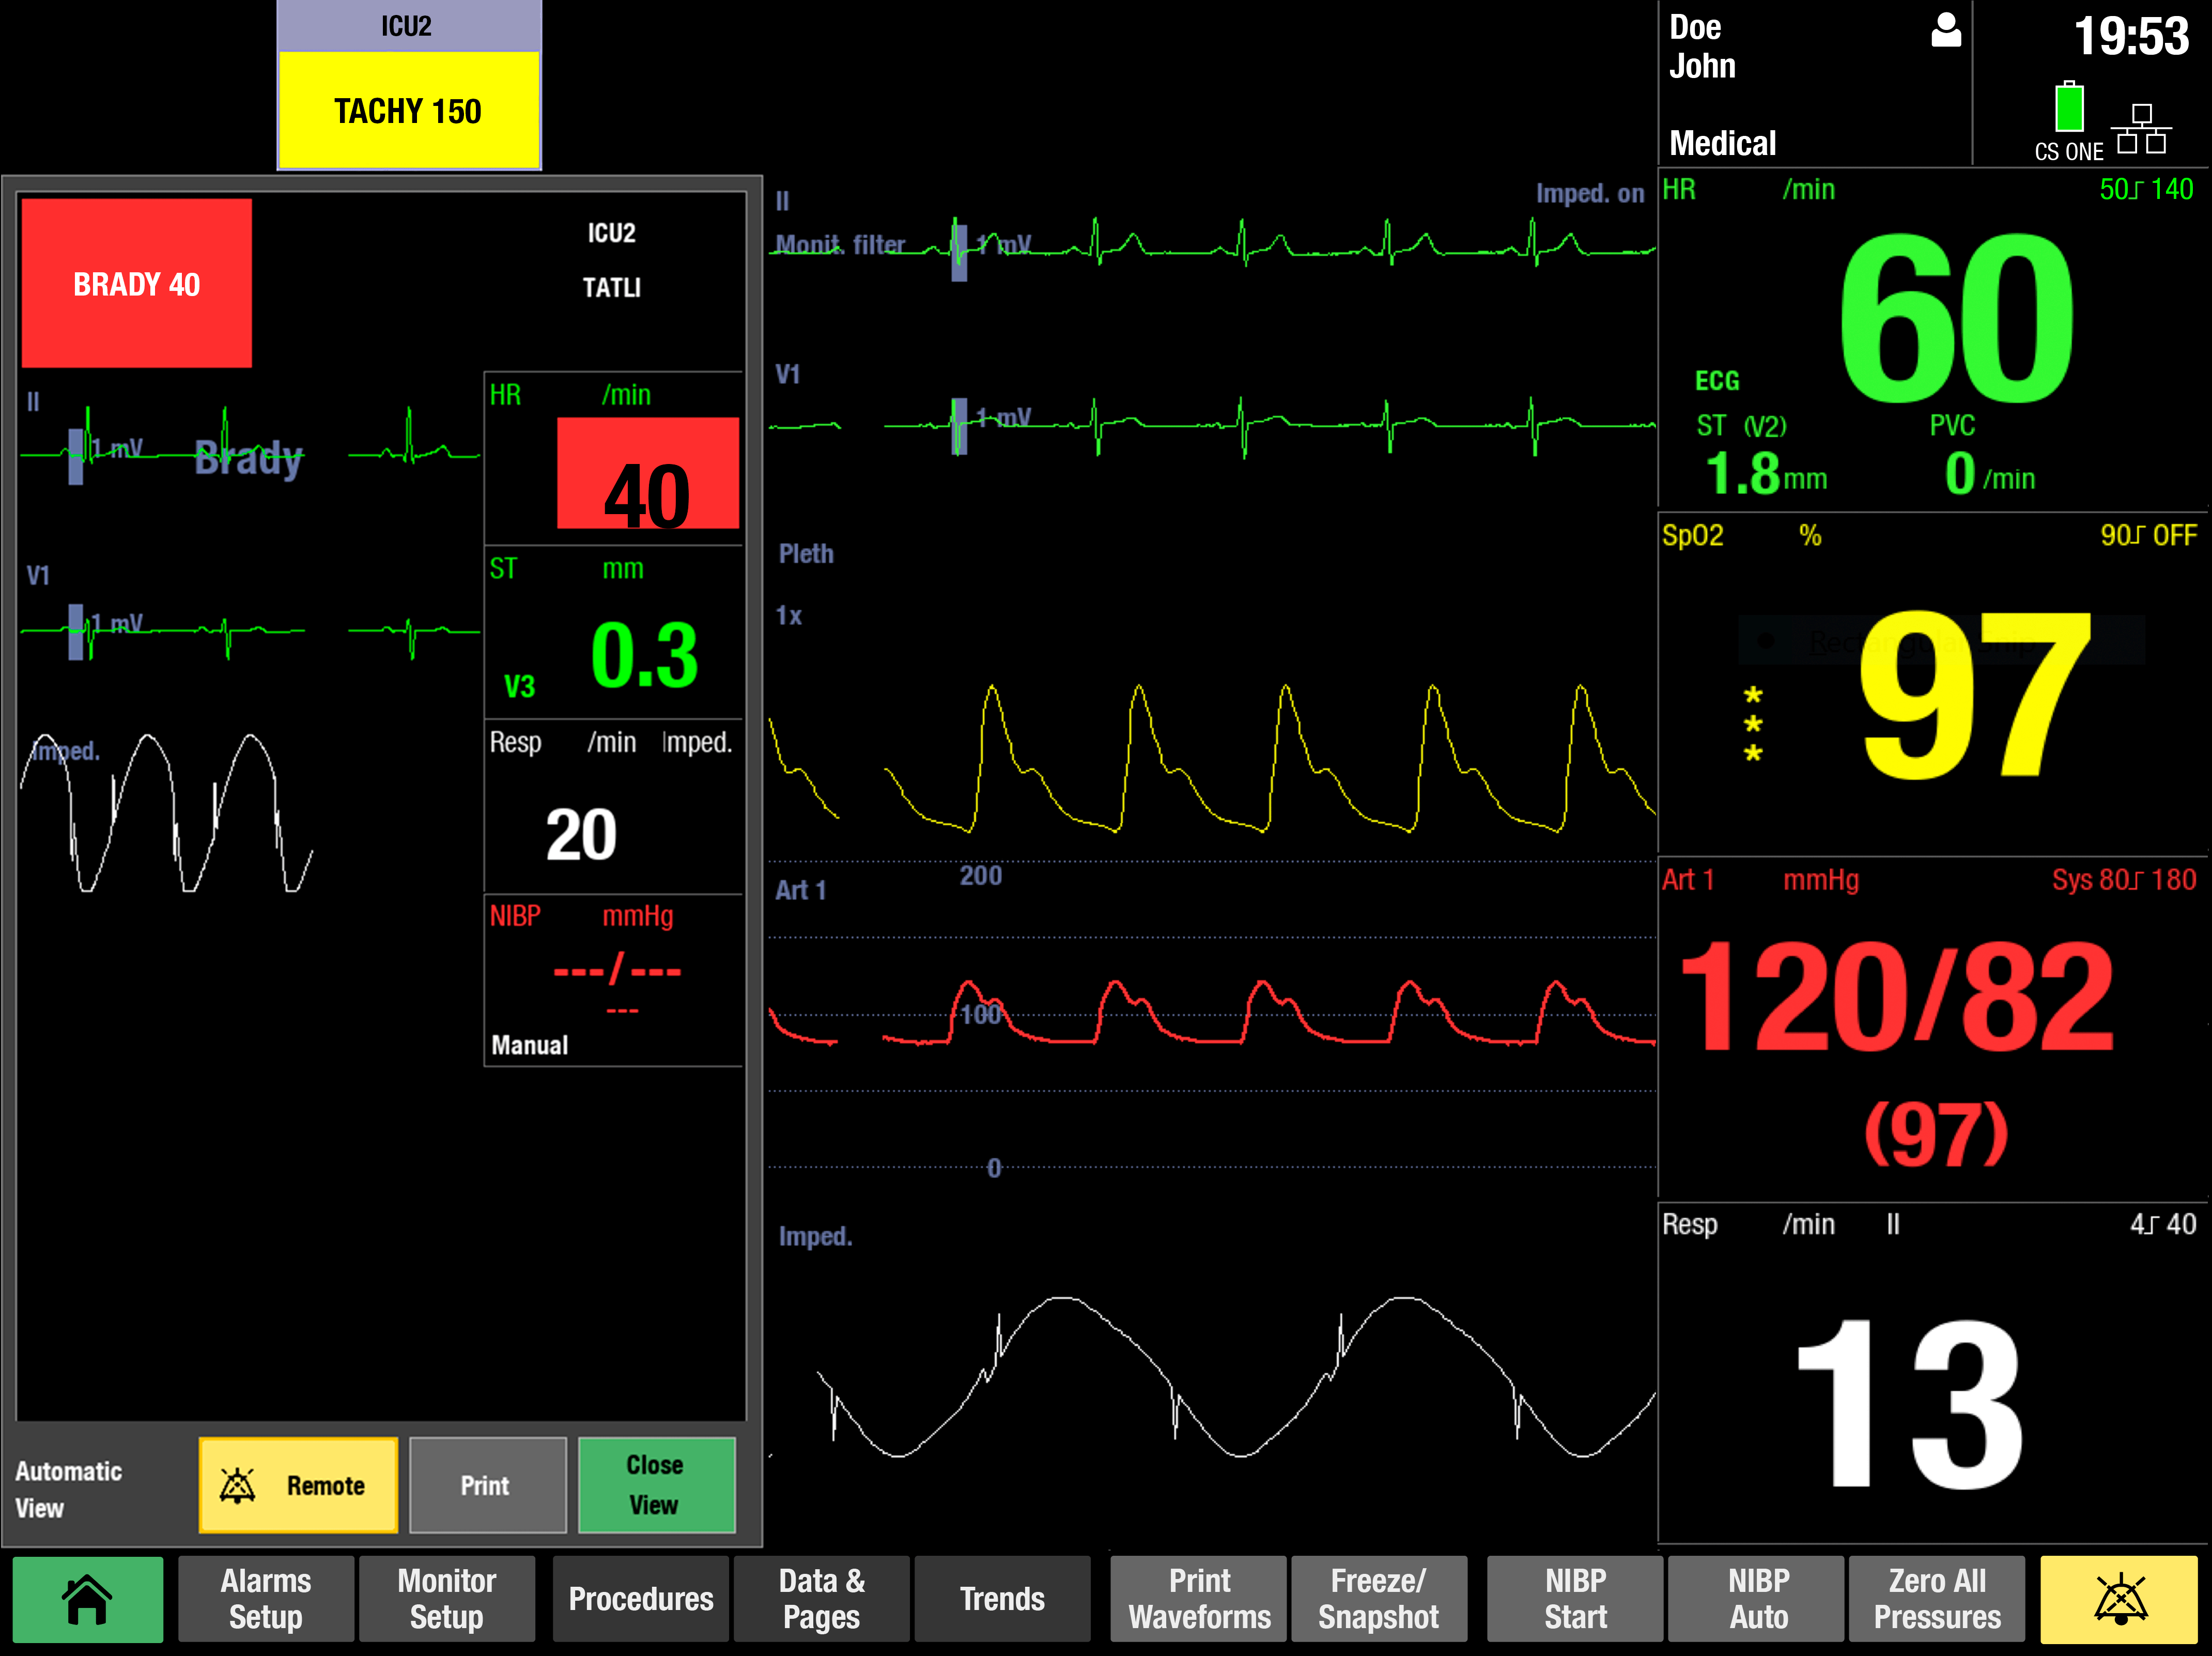
\includegraphics[width=5.5cm]{data_plan/monitor2}
      }
      \caption{\label{fig:monitor}GE Healthcare CARESCAPE B650监护仪}
\end{figure}

\subsection{数据采集规范}
如在绪论PPG原理部分所述,数据采集时选取在被试孕妇的左手食指进行使用透射式血氧探头进行采集。若被试孕妇的左手食指有损伤,则将测量部位替换为左手中指,如\autoref{fig:finger}所示。测量时把手指放入指套内部,
指甲与传感器表面有指甲标记的部位正对,指尖触及但不超出指套顶端,确保发光管发出的所有光线全部通过被试的组织。其中,使用的血氧采集探头美国泰科公司旗下的Nellcor DS-100A型血氧传感器。 
\begin{figure}[htbp]
      \centering
      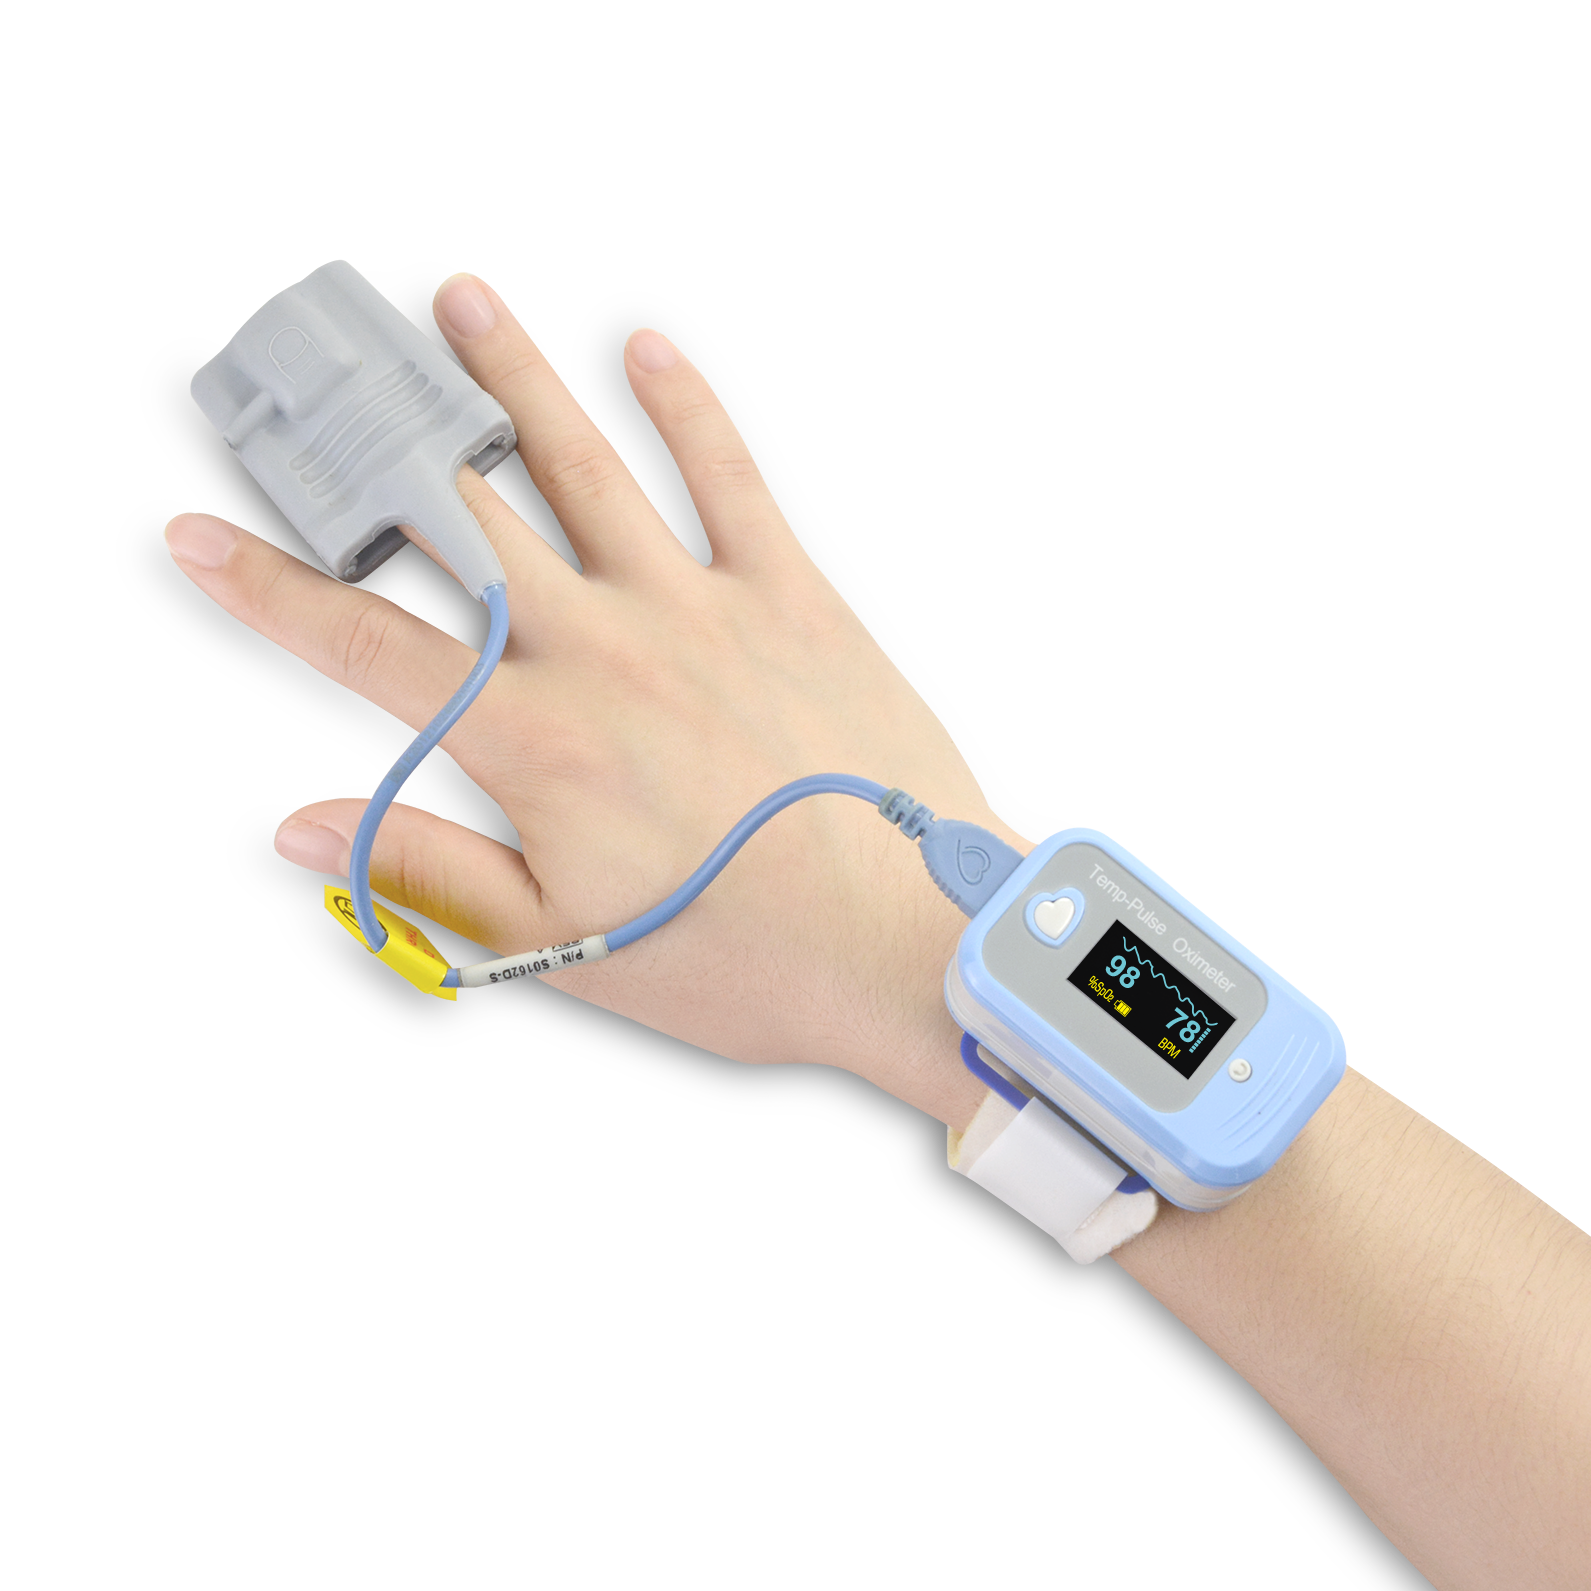
\includegraphics[width=.5\linewidth]{data_plan/finger}
      \caption{\label{fig:finger}血氧采集方式示意}
\end{figure}
\subsection{具体实验流程}
被试人员到达数据实验采集现场后,首先实验人员会登记被试人员包括姓名、年龄、孕产史等一般信息,如\autoref{tab:questionnaire}所示。接着实验人员会告知被试人员本研究的研究背景与实验过程。
在征得被试人员同意后,采集人员会按前文操作规范为被试佩戴血氧采集探头\cite{Chen2021}。
与血压采集过程类似\cite{FIGO},被试人员在实验全程需保持坐姿。在被试孕妇休息至少5分钟后,PPG数据开始正式记录,单次采集时长不低于1分钟。
\subsection{数据导出}
由于GE公司并没有公开B650数据通讯协议,无法直接获取该设备可采集的全部生理参数的原始数据信息。通过产商技术支持提供的第三方软件,可将B650监护仪采集得到的血氧脉搏波数据以(时间-脉搏波相对幅值)键值对的形式以CVS的文件格式导出供后续分析,如\autoref{tab:exporteddata}所示。
其中,导出的PPG信号采样率为100$Hz$。
\subsection{数据复核}
实验期间,本研究共采集得到了80例孕妇的PPG原始数据。经复核校验,有1例正常妊娠孕妇数据因为采集时间过短、信号质量过低等原因被剔除。
最终,79例有效PPG数据进入下一阶段的分析研究,其中实验组患有PE的孕妇有效数据44例,对照组正常妊娠孕妇有效数据35例。
参与被试人员如\autoref{tab:pregnant}所示,被试姓名以姓名全拼缩写代替。
\section{被试孕妇人口统计学特征分析}
尽管\autoref{tab:questionnaire}中设计了与PE相关的多种风险因子的统计,但由于种种原因,只有被试的年龄、孕周、身高、体重、BMI指数、血压及心率等因子可从全部被试孕妇中完整获取。
因此,本小节使用了统计分析的一般方法对被试孕妇的这些人口统计学特征进行了相关分析。
\subsection{变量分析方法}
在对以上风险因子展开分析之前,有必要先介绍下统计分析过程中最常用的工具与方法。

一、相关性分析

相关性分析是指对两个具备相关性的变量元素进行分析,衡量两个变量因素的相关密切程度\cite{Zhang2019}。相关性的元素之间需要存在一定的联系或者概率才可以进行相关性分析。一般可以通过散点图即可直接观察变量之间的联系,如\autoref{fig:relation}所示。
统计学上引入了相关系数$r$以量化表征变量之间的密切程度。$r$的取值范围为[-1,1],其绝对值大小反映了两变量之间相关性的强弱:当$r$>0时,表明两个变量正相关;反之,则两个变量变化趋势相反,呈负相关。

\begin{figure}[htbp]
      \centering
      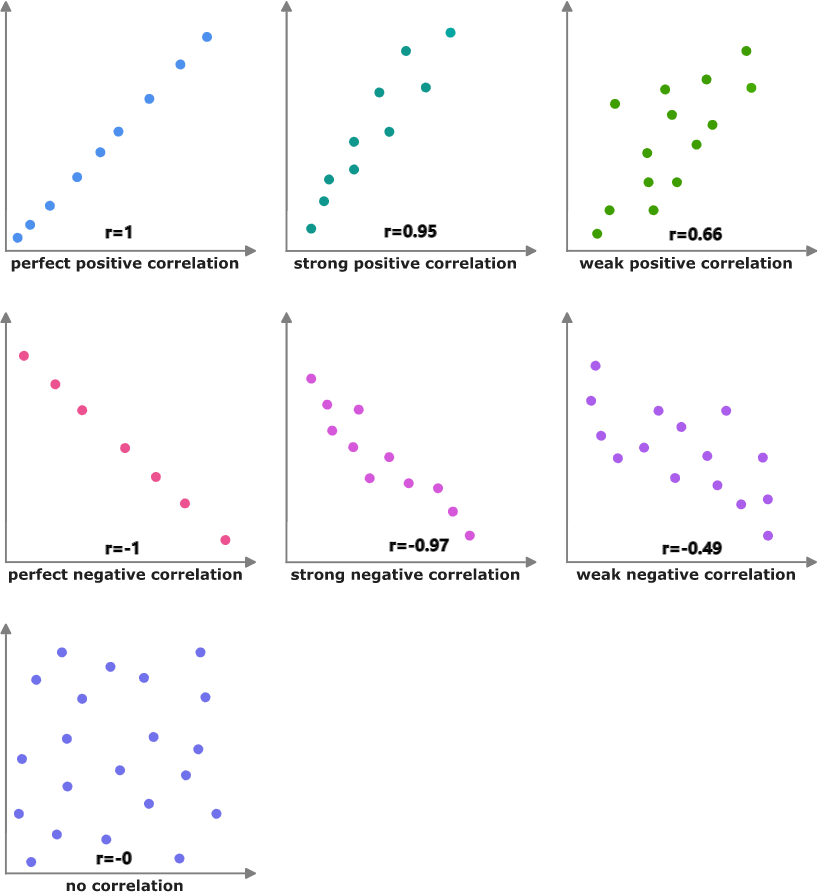
\includegraphics[width=.6\linewidth]{data_plan/relation}
      \caption[二元变量之间常见的相关关系]{\label{fig:relation}二元变量之间常见的相关关系\cite{IXL2022}}
\end{figure}

常用的相关性分析方法有皮尔逊(Pearson)相关性分析法与斯皮尔曼(Spearman)相关性分析法,利用这两种方法计算得到的相关系数也对应被称为皮尔逊相关系数$r_p$与斯皮尔曼相关系数$r_s$:
\begin{equation}
      \label{equ:spearman}
      r_s=1-\frac{6\sum_{i=1}^{n}(x_{i}-y_{i})^2}{n(n^2-1)}
\end{equation}
\begin{equation}
      \label{equ:pearson}
      r_p=\frac{\sum_{i=1}^n{(x_i- \mathop{x} \limits^-)(y_i- \mathop{y} \limits^-)}}{\sqrt{{\sum_{i=1}^n}{{(x_i- \mathop{x} \limits^-)^2\sum_{i=1}^n}{(y_i- \mathop{y} \limits^-)^2}}}}
\end{equation}

一般认为,斯皮尔曼相关性分析适用于对存在单调性关系的变量进行检测,而皮尔逊相关性分析适用于对正态分布的变量进行检测。
由于斯皮尔曼相关系数的计算对变量的分布特性要求并不严格,因而应用得也更为广泛。
如\autoref{equ:spearman}所示,为计算斯皮尔曼相关系数,需要对长度为$n$的待检二元变量$X$与$Y$按升序排列,得到原始数据在排序后的序次$x$、$y$。特别地,若出现多个数据排序相同,则用这些数据的平均序次统一表征后再进行计算。

二、参数检验与非参数检验

数据的集中趋势、离散程度与分布形态是对一组数据进行描述时最常用的三个角度\cite{Hu2021}。而参数检验(parametric test)通常都是在假设数据总体服从正态分布、样本统计量服从T分布的前提下,对总体分布中的总体均值、方差及样本差等未知参数做出统计推断。
而面对总体分布类型未知或分布类型已知,但不对称或变量无法精准测量的数据,或样本容量小、无法运用中心极限定理进行相关参数检验时,
另一类不以特定的总体分布为前提、不针对总体分布参数做任何推断的分析方法也发展起来,此类分析方法被统一称为非参数检验(nonparametric test)\cite{Guo2017,Hu2021,Zhang2019}。

一般而言,参数检验的精确度高于非参数检验,因此在条件允许的情况下,应优先采用参数检验。若由于各种原因导致参数检验的条件不满足,可以应用非参数检验方法对数据进行分析。
常见的非参数检验方法及其适用情形如\autoref{tab:nonparametric-test}所示。
\begin{center}
      \begin{longtable}{m{1.8cm}<{\centering}m{2.5cm}<{\centering}m{5cm}<{\centering}m{6cm}<{\centering}}
		\caption{常见的非参数检验方法}\\
		\label{tab:nonparametric-test}\\
		\toprule
            \textbf{样本数目}&\textbf{样本相关性}&\textbf{检验方法}&\textbf{检验方法英文名}\\
            \midrule
            \endfirsthead
            \caption[]{(续)}\\
            \toprule
            \textbf{样本数目}&\textbf{样本相关性}&\textbf{检验方法}&\textbf{检验方法英文名}\\
            \midrule
            \endhead 
            \hline
            \endfoot
            \bottomrule
            \endlastfoot
            单样本   & /     & 卡方检验  & Chi-Squared Test \\
            单样本   & /     & 二项分布检验 & Binomial Test \\
            单样本   & /     & K-S检验 & Kolmogorov–Smirnov Test \\
            单样本   & /     & 符号秩检验 & Wilcoxon Signed-Rank Test \\
            单样本   & /     & 游程检验  & Wald–Wolfowitz runs Test \\
            两样本   & 独立    & Wilcxon W等级和检验 & Mann-Whitney U Test \\
            两样本   & 独立    & 摩西极端反映差异检验 & Moses Extreme Reaction Test \\
            两样本   & 独立    & K-S检验 & Kolmogorov–Smirnov Test \\
            两样本   & 独立    & 游程检验  & Wald–Wolfowitz runs Test \\
            两样本   & 相关    & 符号检验  & Sign Test \\
            两样本   & 相关    & 符号秩检验 & Wilcoxon Signed-Rank Test \\
            两样本   & 相关    & 变化显著性检验 & McNemar's Test \\
            两样本   & 相关    & 边缘一致性检验 & Marginal Homogeneity Test \\
            多样本   & 独立    & K-W平均秩检验 & Kruskal-Wallis H Test \\
            多样本   & 独立    & 中位数检验 & Median Test \\
            多样本   & 独立    & 分组分布检验 & Jonckheere-Terpstra Test \\
            多样本   & 相关    & 双向等级方差分析 & Friedman Test \\
            多样本   & 相关    & 肯德尔和谐系数检验 & Kendall's W Test \\
            多样本   & 相关    & 二分变量检验 & Cochran's Q Test \\
      \end{longtable}
\end{center}

\begin{table}[htbp]
      \centering
      \caption{\label{tab:factors_res}被试孕妇风险因子统计结果}
      \begin{tabular}{cccc}
      \toprule
      \textbf{检验变量(单位)}      & \textbf{实验组(n=44)} & \textbf{对照组(n=35)} & \textbf{p值} \\
      \midrule
      年龄(years) & 32.3±3.6 & 33.8±4.6 & 0.108 \\
      孕周(weeks) & 32.7±3.8 & 34.3±4.3 & 0.053 \\
      身高(cm) & 158.1±5.0 & 160.0±3.3 & 0.089 \\
      体重(kg) & \textbf{75.7±12.9} & \textbf{67.1±8.2} & 0.002* \\
      BMI(kg/cm) & \textbf{30.2±4.5} & \textbf{26.2±3.3} & <0.001* \\
      收缩压(mmhg) & \textbf{160.1±19.5} & \textbf{111.2±9.8} & <0.001* \\
      舒张压(mmhg) & \textbf{96.1±14.5} & \textbf{66.8±10.4} & <0.001* \\
      心率(bpm) & 87.0±11.9 & 87.5±13.1 & 0.656 \\
      \bottomrule
      \end{tabular}%
\end{table}%
\subsection{分析结果}
在此前数据采集阶段得到的关于所有被试的年龄、孕周、身高、体重、BMI指数、血压及心率等风险因子之间的联系关系等不属于本研究内容,故未作任何相关性分析。而
诸多风险因子等待检参数存在样本量较小、具体分布未知等客观限制因素,故对这些变量的分析均采用了非参数检验中的Wilcxon W等级和检验,亦即Mann-Whitney U检验。
U检验的基本思想是将全部样本混合后一起求秩,然后根据两组样本的秩分情况判断是否存在差异。

被试孕妇涉及的PE风险因子的经U检验后的统计结果如\autoref{tab:factors_res}所示,所有待分析变量均以平均值±标准差的形式表征。从\autoref{tab:factors_res}不难发现,实验组与对照组的被试孕妇在年龄、孕周、身高、心率等风险因子
上均无明显统计意义上的差别(p>0.05),但在收缩压与舒张压的数值上有显著差异(p<0.001),这也与被试孕妇的PE患病状态一致,符合预期。
\section{小结}
本章对本研究涉及的实验数据的来源进行了介绍,从数据采集所使用的实验设备、数据采集规范、数据采集流程与数据导出等角度对数据采集方案进行了详细的说明。在此基础上,本章同时也对被试孕妇的人口统计学特征进行了统计分析,
结果表明,实验组与对照组的被试孕妇中在年龄、孕周、身高、心率等风险因子上均无明显统计意义上的差别,排除了以上因素的对实验结果的干扰。